% // ============================================================================
%//
%// Copyright (c) 1999 The CGAL Consortium
%//
%// This software and related documentation is part of an INTERNAL release
%// of the Computational Geometry Algorithms Library (CGAL). It is not
%// intended for general use.
%//
%// ----------------------------------------------------------------------------
%//
%// release       :
%// release_date  :
%//
%// file          : /doc_tex/basic/Triangulation3/TDS3.tex
%// revision      : $Revision$
%//
%// author(s)     : Monique Teillaud <Monique.Teillaud@sophia.inria.fr>
%//
%// coordinator   : INRIA Sophia Antipolis (Mariette Yvinec <Mariette.Yvinec@sophia.inria.fr>)
%//
%//============================================================================
\chapter{3D Triangulation Data Structure}
\label{chapter-TDS3}

\minitoc

A geometric triangulation has two aspects: the combinatorial structure, which
gives the incidence and adjacency relations between faces, and the
geometric information related to the position of vertices.

\cgal\ provides 3D geometric triangulations in which these
two aspects are clearly separated.
As described in Chapter~\ref{chapter-Triangulation3}, a geometric
triangulation of a set of points in $\R^d$ is a partition of the
whole space $\R^d$ into cells having $d+1$ vertices. Some of them
are infinite, they are obtained by linking an additional vertex at
infinity to each facet of the convex hull of the points (see
Section~\ref{Triangulation3-sec-intro}).  
The underlying combinatorial graph of such a triangulation
without boundary of $\R^d$ can be seen as a triangulation of the
topological sphere $S^d$ in $\R^{d+1}$. 

This chapter deals with 3D-triangulation data structures, meant to
maintain the combinatorial information for 3D-geometric
triangulations. The reader interested in geometric triangulations of
$\R^3$ is advised to read Chapter~\ref{chapter-Triangulation3}.

\section{Representation}
\label{TDS3-sec-intro}

In \cgal, a triangulation data structure is a
container of cells ($3$-faces) and vertices ($0$-faces). Each cell gives
access to its four incident vertices and to its four adjacent
cells. Each vertex gives direct access to one of its incident cells, which is 
sufficient to retrieve all the incident cells when needed.

The four vertices of a cell are indexed with 0, 1, 2 and 3.  The
neighbors of a cell are also indexed with 0, 1, 2, 3 
in such a way that the neighbor indexed by $i$ is opposite to the vertex
with the same index (see Figure~\ref{TDS3-fig-repres}).

\begin{figure}
\begin{ccTexOnly}
\begin{center} 
\includegraphics{repres.eps}
\end{center}
\end{ccTexOnly}
\caption{Representation.
\label{TDS3-fig-repres}}
\begin{ccHtmlOnly}
<CENTER>
<img border=0 src="./repres.gif" align=center
alt="Representation">
</CENTER>
\end{ccHtmlOnly}
\end{figure} 

Edges ($1$-faces) and facets ($2$-faces) are not explicitly
represented: a facet is given by a cell and an index (the facet
\ccc{i} of a cell \ccc{c} is the facet of \ccc{c} that is opposite to
the vertex of index \ccc{i}) and an edge is given by a cell and two
indices (the edge \ccc{(i,j)} of a cell \ccc{c} is the edge
whose endpoints are the vertices of indices \ccc{i} and \ccc{j} of
\ccc{c}). 

\paragraph{Degenerate Dimensions}
As \cgal\ explicitly deals with all degenerate cases, a
3D-triangulation data structure in \cgal\ can handle the cases when
the dimension of the triangulation is lower than~3.

Thus, a 3D-triangulation data structure can store a triangulation of a
topological sphere $S^d$ of $\R^{d+1}$, for any $d \in \{-1,0,1,2,3\}$. 

Let us give, for each dimension, the example corresponding to the
triangulation data structure having a minimal number of vertices, i.e. a 
simplex. These examples are illustrated by presenting their usual
geometric embedding. 
\begin{itemize}
\item \emph{dimension 3.} The triangulation data structure consists of
the boundary of a 4-dimensional simplex, which has 5 vertices. A
geometric embedding consists in choosing one of these vertices to be
infinite, thus four of the five 3-cells become infinite: the geometric
triangulation has one finite tetrahedron remaining, each of its facets
being incident to an infinite cell. See Figure~\ref{TDS3-fig-topo-simplex4}.
\begin{figure}
\begin{ccTexOnly}
\begin{center} 
\includegraphics{topo-simplex4.eps}
\end{center}
\end{ccTexOnly}
\caption{4D simplex and a 3D geometric embedding.
\label{TDS3-fig-topo-simplex4}}
\begin{ccHtmlOnly}
<CENTER>
<img border=0 src="./topo-simplex4.gif" align=center
alt="4D simplex and a 3D geometric embedding">
</CENTER>
\end{ccHtmlOnly}
\end{figure} 
\item \emph{dimension 2.} We have 4 vertices forming one 3-dimensional
simplex, i.e. the boundary of a tetrahedron. The geometric embedding in
the plane results from choosing one of these vertices to be infinite,
then the geometric triangulation has one finite triangle whose edges are
incident to the infinite triangles. See Figure~\ref{TDS3-fig-topo-simplex3}.
\begin{figure}
\begin{ccTexOnly}
\begin{center} 
\includegraphics{topo-simplex3.eps}
\end{center}
\end{ccTexOnly}
\caption{3D simplex and a 2D geometric embedding.
\label{TDS3-fig-topo-simplex3}}
\begin{ccHtmlOnly}
<CENTER>
<img border=0 src="./topo-simplex3.gif" align=center
alt="3D simplex and a 2D geometric embedding">
</CENTER>
\end{ccHtmlOnly}
\end{figure} 
\item \emph{dimension 1.} A 2-dimensional simplex (a triangle) has 3
vertices. The geometric embedding is and edge whose vertices are linked
to an infinite point.  See Figure~\ref{TDS3-fig-topo-simplex2}.
\begin{figure}
\begin{ccTexOnly}
\begin{center} 
\includegraphics{topo-simplex2.eps}
\end{center}
\end{ccTexOnly}
\caption{2D simplex and a 1D geometric embedding.
\label{TDS3-fig-topo-simplex2}}
\begin{ccHtmlOnly}
<CENTER>
<img border=0 src="./topo-simplex2.gif" align=center
alt="2D simplex and a 1D geometric embedding">
</CENTER>
\end{ccHtmlOnly}
\end{figure} 
\end{itemize}

The last three cases are defined uniquely:
\begin{itemize}
\item \emph{dimension 0.} A 0-dimensional triangulation is
combinatorially equivalent to the boundary of a 1-dimensional simplex
(an edge), which consists of 2 vertices. One of them becomes infinite
in the geometric embedding, and there is only one finite vertex
remaining. The two vertices are adjacent.
\item \emph{dimension -1.} This dimension is a convention to represent a 
0-dimensional simplex, that is a sole vertex, which will be
geometrically embedded as an ``empty'' triangulation, having only one
infinite vertex.
\item \emph{dimension -2.} This is also a convention. The
triangulation data structure has no vertex. There is no associated
geometric triangulation.
\end{itemize} 

Note that the notion of infinite vertex has no meaning for the
triangulation data structure. The infinite vertex of the geometric
embedding is a vertex that cannot be distinguished from the other
vertices in the combinatorial triangulation.

The same cell class is used in all cases: triangular faces in
2D can be considered as degenerate cells, having only three vertices
(resp. neighbors) numbered $(0,1,2)$;
edges in 1D have only two vertices (resp. neighbors) numbered $0$ and $1$.

The implicit representation of facets (resp. edges) still holds
for degenerate ($< 3$) dimensions : in dimension~2, each cell has only one
facet of index 3, and 3 edges $(0,1)$, $(1,2)$ and $(2,0)$; in
dimension~1, each cell has one edge $(0,1)$. 

\paragraph{Validity}
A 3D combinatorial triangulation is said to be \ccc{locally valid} 
iff the following is true:

{\bf (a)} When a cell $c$ has a neighbor pointer to another cell $c'$,
then reciprocally this cell $c'$ has a neighbor pointer to $c$, and
$c$ and $c'$ have three vertices in common. These cells are called
adjacent. 
% Two adjacent cells have reciprocal neighbor pointers to each
% other and they have three vertices in common. 

{\bf (b)} The cells have a coherent orientation: if two cells $c_1$
and $c_2$ are adjacent and share a facet with vertices $u,v,w$, then
the vertices of $c_1$ are numbered $(v_0^1 = u, v_1^1 = v, v_2^1 = w,
v_3^1)$, and the vertices of $c_2$ are numbered $(v_0^2 = v, v_1^2 = u,
v_2^2 = w, v_3^2)$, up to positive permutations of $(0,1,2,3)$. In
other words, if we embed the triangulation in $\R^3$, then the fourth
vertices $v_3^1$ and $v_3^2$ of $c_1$ and $c_2$ see the common facet
in opposite orientations. See Figure~\ref{TDS3-fig-comborient}.

The set {\Large $\sigma$}$_4$ of permutations of
$(0,1,2,3)$ has cardinality 24, and the set of positive permutations
$A_4$ has cardinality 12. Thus, for a given orientation, there
are up to 12 different orderings of the four vertices of a cell. Note
that cyclic permutations are negative and so do not preserve the
orientation of a cell.

\begin{figure}[htbp]
\begin{ccTexOnly}
\begin{center} 
\includegraphics{comborient.eps} 
\end{center}
\end{ccTexOnly}
\caption{Coherent orientations of two cells (3-dimensional case).
\label{TDS3-fig-comborient}}
\begin{ccHtmlOnly}
<CENTER>
<img border=0 src="./comborient.gif" align=center alt="Orientation of a cell (3-dimensional case)">
</CENTER>
\end{ccHtmlOnly}
\end{figure} 

The \ccc{is_valid()} method provided by
\ccc{Triangulation_data_structure_3} checks the local validity of a
given triangulation data structure.
 
\section{Software Design}
\label{TDS3-sec-design}

The 3D-triangulation data structure class of CGAL is designed to be
used as a combinatorial layer upon which a geometric layer can be
built \cite{k-ddsps-98}. This upper class can be the 3D-triangulation
class of \cgal. Figure~\ref{TDS3-fig-layers} shows the organization of
the software design in this case.

\begin{figure}[htbp]
\begin{ccTexOnly}
\begin{center} 
\includegraphics{design.eps} 
\end{center}
\end{ccTexOnly}
\caption{Layers in the software design.
\label{TDS3-fig-layers}}
\begin{ccHtmlOnly}
<CENTER>
<img border=0 src="./design.gif" align=center alt="Layers in the software design">
</CENTER>
\end{ccHtmlOnly}
\end{figure} 

In the bottom layer, the base classes store elementary
geometric information.  These classes are parameterized by a geometric
traits class providing all the geometric types. A vertex stores a cell handle,
and a cell stores four vertex handles and four cell handles.

The middle layer class stores the triangulation data structure, which
is purely combinatorial.  The triangulation data structure provides
operations such as insertion of a new vertex in a given cell, on a
$1$ or $2$-face. It also allows one, if the dimension of the triangulation
is smaller than $3$, to insert a vertex so that the dimension of the
triangulation is increased by one. The triangulation data
structure is responsible for the combinatorial integrity of the
triangulation. 

It is up to the user to derive his own base classes from the \cgal\
base classes to add any other information he may need for his given
application, or to write his own base classes from scratch. In this
case, the base classes must be models for the \ccc{TriangulationVertexBase_3}
and \ccc{TriangulationCellBase_3} concepts described in
\ccRefPage{TriangulationVertexBase_3} and \ccRefPage{TriangulationCellBase_3}.

The upper layer, described in Chapter~\ref{chapter-Triangulation3}, is
the geometric triangulation class, providing operations such as
location of a point in the triangulation, insertion of a point, and is
responsible for the geometric validity.  The triangulation
data structure class is one of the template parameters of the
geometric triangulation class. The user may choose to replace the
triangulation data structure class provided by \cgal\ by his own triangulation
data structure. In this case, his class has to be a model of the
\ccc{TriangulationDataStructure_3} concept described in
\ccRefPage{TriangulationDataStructure_3}.

\section{Example of incremental construction}
\label{TDS3-sec-examples}
The following example shows how to construct a 3D triangulation data
structure by inserting vertices.

\ccIncludeExampleCode{Triangulation_3/example_tds.C}
